\section{Anwendungsbezogene Kriterien}
\label{sc:AnwendungsbezogeneKriterien}
Anwendungsbezogene Kriterien beschreiben die Anforderungen einer Modellierungssprache an eine Anwendung innerhalb eines Domänenspezifischen Einsatzes.
Dies hängt von den jeweiligen Aspekten ab, welche durch die Modellierungssprache abgebildet werden soll.
So besitzen verschiedene Modellierungssprachen unter anderem ein unterschiedlich großes Nutzungspotenzial in der jeweiligen Anwendungsdomäne.
Man spricht in diesem Zusammenhang auch von der Mächtigkeit der Sprache.
Dabei ist zu beachten, das Anwendungs- und Anwenderbezogene Kriterien oft konkurrierend sein können,
so kann sich beispielsweise eine leicht erlernbare Sprache sich negativ auf die Mächtigkeit auswirken und umgekehrt.
Anwendungsbezogene Kriterien können in Anforderungen wie der Angemessenheit, der Mächtigkeit, der Operationalisierbarkeit,
und der Überprüfbarkeit beschrieben werden.
Zwar gibt es höchstwahrscheinlich noch eine weit aus größere Anzahl an Kriterien, diese sollen uns aber in dieser Arbeit genügen \cite[95\psq]{JaneFroeming_2009}.
\subsection{Angemessenheit}
\label{ssc:Angemessenheit}
Die Angemessenheit einer Sprache bezieht sich auf die Gesamtheit der Sprache,
als auch auf die einzelnen Konzepte der Sprache und umfasst damit das Abstraktionsniveau, den Detaillierungsgrad und den Formalisierungsgrad einer Sprache \cite[97]{Lobe_2015}.

Die Abstraktionsfähigkeit einer Modellierungssprache beschreibt, worin die Fachterminologie der Domäne sich mit den Konzepten der Modellierungssprache möglichst decken sollte und welche unwesentlichen Details abstrahiert werden. In dem Bereich von Kommunikationsabläufen der Telekommunikation sind diese Begriffe eher technischer Natur und kommen aus einem Informatik-spezifischem Umfeld, welcher Fachsprache auf dem Niveau von Spezialisten voraussetzt. 

Der Detaillierungsgrad beschreibt wie Sachlich angemessen detailliert die Konstrukte eines Anwendungszwecks der Domäne sich darstellen lassen können. Dies beinhaltet die zu Modellierenden Modelle, Daten und zusätzlichen Informationen. Damit ist nicht gemeint, dass ein System in einer hohen Abstraktionsform eine eins zu eins Nachbildung aller technischen Prozesse des Informationssystems ausdrücken soll,
sondern nur für die Zielgruppe angemessene und verständliche Konzepte. Eine formale Beschreibung der Prozesse ist demnach nicht gewünscht, da der Hauptaugenmerk auf dem Anwender liegt.

Die Angemessenheit der Sprache ist abhängig durch den Anwendungszweck.
Da aber der Sachverhalt zumeist unklar definiert ist, ist es nicht immer möglich zu überprüfen ob ein Modell einen Sachverhalt abbildet. Dies ist nicht der Fall, wenn der Sachverhalt exakt definiert ist und eine formale Überprüfung der Angemessenheit vorgenommen werden kann.

Genauso steht sie somit in direktem Zusammenhang mit der Mächtigkeit, einem weiterem Kriterium, welche später in der Arbeit behandelt wird und dem Anwendungszweck einer Sprache. 
So bieten Angemessenheit und Mächtigkeit zusammen die Möglichkeit, die bereitgestellten Konzepte einer Sprache bezogen auf den Anwendungszweck zu untersuchen. Demnach sollen ausreichende Konzepte bereitgestellt werden, ohne jedoch überflüssige Konzepte zu enthalten \cite[35F]{Frank_1997}.

\subsubsection{Konsequenz}
Im Hinblick ob ein Konstrukt der Sprache nun Angemessen ist oder nicht, hängt subjektiv vom jeweiligen Betrachter ab. 
Dies ist insbesondere bei komplizierten Konstrukten Fall. Im Zweifelsfall muss nun entschieden werden, ob es ein notwendiges Sprachkonstrukt darstellt oder ob es nur die Sprachkomplexität erhöht. Dies muss jedoch für jedes einzelne Konstrukt abgewägt werden, da jedes seine eigenen spezifischen Vor- und Nachteile besitzt. Laut Ulrich Frank und Micheal Prasse ist es sogar gar nicht möglich, ein formelles Maß zu Bestimmung von Angemessenheit von Modellierungssprachen zu besitzen, da die Untersuchung eines Konstrukts der Sprache immer nur subjektiv erfolgen kann, man jedoch aber die Bedeutsamkeit des Konstrukts im jeweiligen Anwendungsfalls beurteilen kann \cite[35]{Frank_1997}.

\subsection{Mächtigkeit}
\label{ssc:Nutzungspotenzial}
Die Mächtigkeit ist ein maß des Nutzungspotenzials einer Sprache und gibt Aussage darüber,
in wie weit und wie gut die Konzepte der verwendeten Sprache, die Eigenschaften eines Sachverhalt der Domäne darstellen kann.
Darunter fällt wie Präzise diese Aussagen sind und wie hoch der Detailgrad der darzustellenden Eigenschaft ist \cite[180]{Allweyer_2005}.
Der Sprachumfang korreliert mit der Mächtigkeit der Sprache. Je größer dieser Umfang ist, desto größer ist auch die Mächtigkeit der Sprache.
Da es für den Anwender von großer Bedeutung ist, seine Anwendung mit einem möglichst umfänglichen Detailgrad beschreiben zu können,
muss die Mächtigkeit mindestens alle Aspekte enthalten, die für den gewünschten darzustellenden Sachverhalt notwendig sind.
Eine Mächtigkeit der Sprache, die sich über den Anwendungszweck der Domäne bezieht, kann wie schon erwähnt sich negativ auf andere Kriterien auswirken.
Ferner jedoch, kann man die Mächtigkeit einer formalen Modellierungssprache in der Automatentheorie anhand ihres Grammatik-Typen festlegen.
Eine Modellierungssprache sollte sich auf die Modellierung konzentrieren.
So können zu viele Konzepte zu einer unangemessen mächtigen Sprache führen, was zwangsläufig ihre Komplexität erhöht. Zwischen Mächtigkeit
und Angemessenheit muss daher ein ausgewogenes Verhältnis existieren.

\subsubsection{Konsequenz}
Mächtigkeit und Angemessenheit bedingen einander. Die Mächtigkeit einer Sprache muss daher relativ
zur Anwendungsdomäne betrachtet werden. Geht man grundsätzlich davon aus, dass die hier betrachteten
Modellierungssprachen der konzeptuellen Modellierung dienen, misst sich die Mächtigkeit einerseits
an der Möglichkeit, als wesentlich erkannte Sachverhalte des abzubildenden Realitätsbereichs
natürlich, also ohne aufwendige Rekonstruktionen, beschreiben zu können. Andererseits sollte die
Modellierungssprache auch Möglichkeiten bieten, Informationen darzustellen, die für die Implementierung
benötigt werden.


\subsection{Operationalisierbarkeit}
\label{ssc:Operationalisierbarkeit}
Die Operationalisierbarkeit gibt Aussage darüber, ob und wie gut sich die Modellierungssprache über ihre eigene Verwendung hinaus noch weiter verwenden lässt.
Darunter fällt die Transformation des Modells in andere Sprachen als auch das darstellen von diversen Sachverhalten.
Bei der Transformation ist hierbei zu beachten, dass die verwendeten Konzepte beider Sprachen möglichst gleich sein müssen,
um eine annähernd vollständige Konvertierung zu ermöglichen. Zur Abbildung diverser Sachverhalte enthält eine gute Operationalisierbarkeit die Abbildungsmöglichkeit von Funktionen, Bedingungen, Ressourcen, Objekten und Ereignissen.
Deswegen müssen Konzepte zur Planung und Analyse des domänenspezifischen Einsatzes enthalten sein \cite[95\psq]{JaneFroeming_2009}.

\subsection{Überprüfbarkeit}
Die Überprüfbarkeit eines Modells einer Modellierungssprache bezieht sich auf die Realitätsnähe eines abzubildenden Sachverhalts. Es ist also ein Maß der Abweichung eines Modells, bezogen auf die Realität welches es abbilden soll.
Ein Modell sollte also immer möglichst genau, überprüfbar und nachvollziehbar an der Realität übergreifend für die Betrachter liegen. Dabei muss jedoch berücksichtigt werden, dass objektive Verfahrensweisen für ein Modell nicht vollumfänglich anwendbar sind, da es sich meist um geplante und nicht faktischen Realitäten handelt. Dadurch gegeben obliegt diese Einschätzung  dann den Betrachter des Modells. Sollten diese einen Konsens über die geplanten Erwartungen erreichen, so kann ein Modell als realistisch eingeschätzt werden \cite[3]{Becker_2012}. Bei der objektive Überprüfung ist die Semantik einer Sprache zu prüfen, dabei ist zwischen den formalen und informalen Sprachen zu unterscheiden. Da ein Modell eine abstrakte Abbildung eines Sachverhalts darstellt, werden in ihm nur die wesentlichen Eigenschaften berücksichtigt und nicht Sachbezogene Eigenschaften ausgelassen. Abbildung \pageref{fig:Beziehung} zeigt die Beziehung zwischen Modell und abzubildender Sachverhalt.
\begin{center}
	\begin{figure}[h]
		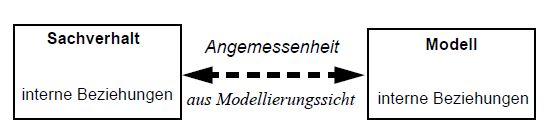
\includegraphics[scale=1]{Graphics/Sachverhalt.jpg}
		\captionof{figure}{Beziehung zwischen Modell und zu modellierendem Sachverhalt, Quelle : \cite[35]{Frank_1997}}
		\label{fig:Beziehung}
	\end{figure}
\end{center}
Sollte ein Modell nicht formal definiert sein, so ist die einzige Möglichkeit, den Inhalt dessen zu erfassen und mit dem gegebenen Sachverhalt entgegen zu prüfen. Je nachdem wie exakt und präzise ein Modell interpretiert werden kann, desto leichter kann es mit dem abzubildenden Sachverhalt verglichen werden. Es ist zwar prinzipiell nicht zu entscheiden, ob ein unpräziser Sachverhalt und ein präzises Modell adäquat sind, jedoch hilft die Präzession und Genauigkeit eines Modells bei dem Vergleich des abzubildenden Sachverhalts. Eine Modellierungssprache, die es ermöglicht, Modelle exakt und eindeutig zu beschreiben
und zu interpretieren, erleichtert daher die Überprüfung des Modells wesentlich. Ist das Modell eindeutig, so ist auch ein umfängliches übergreifendes Verständnis möglich. Dies bedeutet aber auch, das jedes Sprachkonstrukt und Sprachverhalten eindeutig interpretiert werden muss. Ansonsten kann dies wegen Interpretationsschwierigkeiten zu Missverständnissen führen. Deswegen muss eine abstrakten Syntax und Semantik vorausgesetzt werden, um die Interpretation der Modelle zu vereinheitlichen \cite[35F]{Frank_1997}.
